% template created by: Russell Haering. arr. Joseph Crop
\documentclass[12pt,letterpaper]{article}
\usepackage{anysize}
\usepackage{cite}
\usepackage{amsmath,amssymb,amsfonts}
\usepackage{algorithm}
\usepackage[noend]{algpseudocode}
\usepackage{graphicx}
\usepackage{multirow}
\usepackage{listings}
\usepackage{xcolor}


\marginsize{2cm}{2cm}{1cm}{1cm}

\lstset{ framexleftmargin=9mm, frame=shadowbox,tabsize = 4}

\begin{document}

\begin{titlepage}
    \vspace*{4cm}
    \begin{flushright}
    {\huge
        ECE 375 Lab 4\\[1cm]
    }
    {\large
    	Large Number Arithmetic
    }
    \end{flushright}
    \begin{flushleft}
    Lab session: 015
    
    Time: 12:00-13:50
    \end{flushleft}
    \begin{flushright}
    Author: Astrid Delestine

    Programming partner: Lucas Plastid 

    \vfill
    \rule{5in}{.5mm}\\
    TA Signature
    \end{flushright}

\end{titlepage}

\section{Introduction}
%This is the first Lab in the ECE 375 series and it covers the setup and compilation of an AVR Assembly Program. The student will learn how how to use the sample Basic Bump Bot assembly file and send the binaries to the AVR Microcontroller board. For the second part of the lab the student will be expected to download and compile the included C sample program and from it learn how to configure the I/O ports of the ATmega32U4 Microcontroller. The student will then write their own C program and upload it to the Microcontroller to verify that it runs as expected. The provided programs have been attached in the source code section of this report.
This is the fourth lab in the ECE 375 series and it covers adding and subtracting words as well as multiplying words together. In this sense words designate 16 bit numbers. It is important to note that this assembly was written for the m128 chipset and not the regular atmetga32u4 chipset. This is due to the fact that we can operate a simulation tool when using the m128 chipset that is not available when we use our regular chipset. The student will write their assembly to do these expected operations with large numbers and is given the expected inputs and can calculate the outputs.

\section{Design}
This lab Lucas and I collaborated and built out ideas for multi-byte addition, subtraction, and multiplication. It was quite interesting to see our ideas collide and how different approaches can be taken to the same problem. Addition can be considered very trivial, however subtraction becomes a little more difficult as the programmer has to consider negative values and if they are possible with this code. In the handout it clearly states that in this lab we will only be dealing with a more simple unsigned subtraction so the result can be held in two 8 bit registers. Next the multiplication of two 24 bit numbers. This will be more difficult than the previous two problems. In this case we decided to solve the problem linearly and not worry about looping or recursion. Finally we move on to the compound function, which uses each of the previously implemented methods to solve the problem of \(((G-H)+I)^2\). 

\begin{figure}[h]
	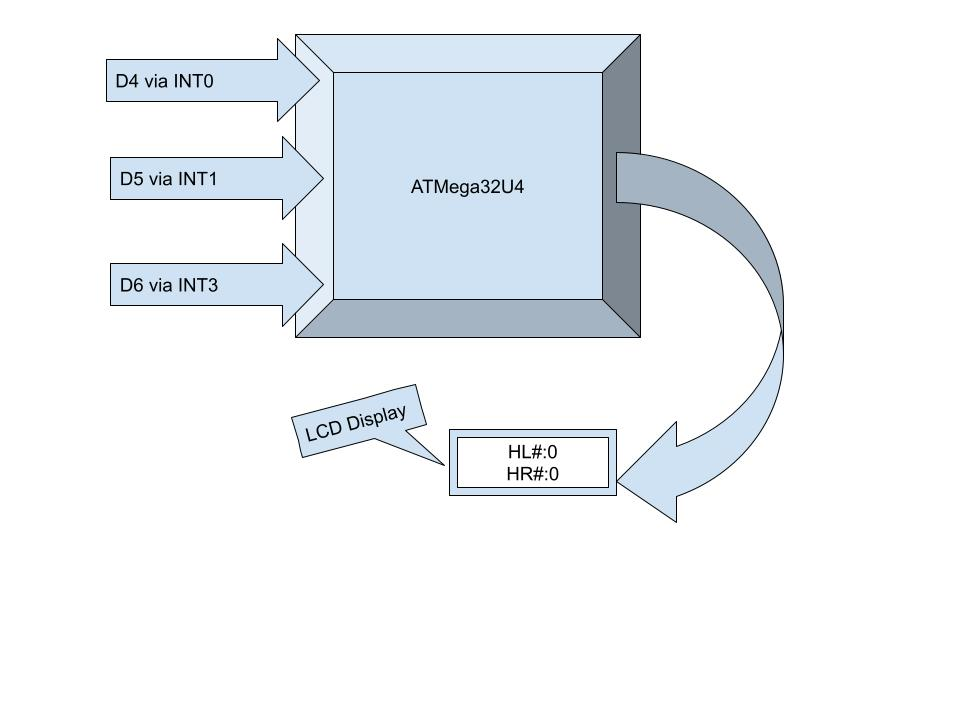
\includegraphics[width=12cm, height=10cm]{Block Diagram L5.jpg}
	\centering
\end{figure}
	
\section{Assembly Overview}
As for the Assembly program an overview can be seen below. It is also important to note that for each of the subroutines all the registers used are pushed and popped to and from the stack unless otherwise stated.

\subsection{Internal Register Definitions and Constants}
The multipurpose register was setup as r16. At r0 and r1 any multiplication output will be set, such that the outputs of any multiplication operation are automatically assigned to them. A default zero register is set to r2. Two other generic variable registers are defined as r3 and r4. Finally two registers named oloop and iloop are used for counting within the assembly itself.

\subsection{Initialization Routine}
Firstly the stack pointer is initialized, then the register defined above as the zero register is cleared.

\subsection{Main Routine}
The main operations that happen in the main routine are those that are initialized below and are called in this order. Firstly the adding operations take place, those being LOADADD16 and ADD16. Next the functions associated with the subtraction operation are called, those being LOADSUB16 and SUB16. Next the functions referencing the MUL24 operation are called. In order they are called LOADMUL24 and MUL24. Finally the compound function set is called, being LOADCOMPOUND and COMPOUND. Once all of these functions have been called the main method loops at the done flag, determining the program to be complete.


\subsection{Subroutines}
	\subsection{ADD16}
	This subroutine adds two 16 bit numbers together. It does this by taking each X Y and Z registers and setting them to operator 1 operator 2 and the location to save the result respectively. Next, using the A variable register as an intermediary the two inputs were added together and saved into the Z register location. Finally if the carry flag is set at the end of the whole operation then we can assume the most significant bit needs to be set to 1, so it is done. 
	
	\subsection{SUB16}
  	This subroutine takes two different inputs and subtracts the first from the second. The X Y and Z registers are initialized at the beginning of this subroutine first, the same way that they are in the add subroutine. In the actual operation part of this subroutine A and B registers are loaded with the lower values of X and Y and subtracted from each other. This is then preformed again to account for the second word. Due to the fact that we do not need to worry about signage these are each saved directly to the location pointed to by Z 

	\subsubsection{MUL24}
	This subroutine takes 4 different data locations and multiplies 24 bits by 24 bits, resulting in a 48 bit number. It must be built differently to the MUL16 operation. Every time addition occurs  we need to check for the carry bit and pass it forward if necessary. This will continue until there is no carry bit to pass upward. In reality this can only ever happen up to 4 times. In this subroutine the first operand is loaded into the Z pointer. Then the second operand is loaded into the Y pointer, finally the result is loaded into the X register. For each of these, they load the start of each because they will increment throughout the method. The data in Y an Z are multiplied and the result is stored in r0 and r1. ADDMUL2x is then called. This fixes the carry bit problem of multiplying by 24 bits and as long as we call ADDMUL2x after our multiplication then everything will work out. 
	 
	
	\subsubsection{ADDMUL2x}
	This subroutine adds a partial multiplication result to the location x is pointing to. This presumes that x is already pointing to the location where the low result of the current multiplication needs to go. Essentially it takes the multiplication outputs and cycles the carry bit up until it cannot anymore. It utilized a loop moving the carry byte in and out of X when necessary.
	
	\subsubsection{COMPOUND}
	Preforms the operation \(((G-H)+I)^2\) Using multiplication, addition and subtraction.
	
	\subsubsection{CLRRES}
	Clears the result memory locations for each ADD16 SUB16 and MUL24. Makes heavy use of the zero register
	
	\subsubsection{LOADMUL24, LOADADD16, LOADSUB16, \& LOADCOMPOUND}
	These subroutines have all been combined as they all do essentially the same operation, they just differ in the data they point to. They load all of the numbers used in each subroutine called above from data memory into program memory so that they are more easily accessible. 
	
	\subsubsection{MUL16}
	A pre-supplied basis subroutine that multiplies 2 16 bit numbers together. 
	
	\subsubsection{FUNC}
	A pre-supplied boiler plate function template that each subroutine is based off of.

\section{Testing}
Tested Each input value and compared to external calculations.
\begin{table}[h]
	\centering
	\begin{tabular}{|l|l|l|ll}
		\cline{1-3}
		Case & Expected & Actual meet expected &  &  \\ \cline{1-3}
	\( \$FCBA + \$FFFF \) 	&\$01FCB9&	\checkmark  &  \\ \cline{1-3}
	\( \$FCB9 - \$E420 \)	&\$1899&	\checkmark	&  \\ \cline{1-3}
	\( \$00FFFFFF * \$00FFFFFF \)	&\$FFFFFE000001&	\checkmark  &  \\ \cline{1-3}
	\(((\$FCBA-\$2022)+\$21BB)^2\)	&\$FCA8CEE9&	\checkmark	&  \\ \cline{1-3}
	
%		&          &                      &  &  \\ \cline{1-3}
	\end{tabular}
\caption{Assembly Testing Cases}
\end{table}

\section{Study Questions}
\begin{enumerate}
    \item
    Although we dealt with unsigned numbers in this lab, the ATmega32 micro-controller also has some features which are important for performing signed arithmetic. What does the V flag in the status register indicate? Give an example (in binary) of two 8-bit values that will cause the V flag to be set when they are added together.
    
    The V flag is the 2's complement overflow indicator, this would be useful when two negative values are being added or subtracted for example 0b1000\_0000 - 0b1000\_0000. This result would no longer fit in the 2's complement space, and so the V flag would be thrown
    
    
    \item 
    In the skeleton file for this lab, the .BYTE directive was used to allocate some data memory locations for MUL16’s input operands and result. What are some benefits of using this directive to organize your data memory, rather than just declaring some address constants using the .EQU directive?
    
    Using the .BYTE directive allows you to not only assume the space is empty but also it allows you to pre-allocate a size of the space that .equ does not.
    
    
    \item 
    In computing, there are traditionally two ways for a microprocessor to listen to other devices and communicate: polling and interrupts. Give a concise overview/description of each method, and give a few examples of situations
    where you would want to choose one method over the other.    
    
    Polling is essentially when the computer is constantly asking a device for its status. This might be good when plotting a data stream that is constantly flowing into the computer. Interrupts allow the computer to work on other tasks and if a button or certain signal is received, it stops whatever it is doing, goes and runs the triggered task, and returns to whatever it was doing prior. This would be very good for a mouse and keyboard. 
    
    \item
	Describe the function of each bit in the following ATmega32U4 I/O registers: EICRA, EICRB, and EIMSK. Do not just give a brief summary of these registers; give specific details for each bit of each register, such as its possible values and what function or setting results from each of those values. Also, do not just directly paste your answer from the datasheet, but instead try	to describe these details in your own words.
	
	in EICRA bits 0 and 1 determine if the signal is detected on a rising edge, falling edge, any edge, or a low level. These control the first 4 interrupts in a fashion such that interrupt 0 is the 0th and 1st bits, interrupt 1 is the 2nd and 3rd bits, and so on. EICRB is very similar except it only handles external interrupt 6, on its 4th and 5th bits. all of its other bits are reserved. EIMSK is an interrupt mask, to enable an interrupt it must be enabled here, the interrupt is associated with its bit, ie bit 6 masks for interrupt 6. This is active high.
	
	
    
	\item 
	The ATmega32U4 microcontroller uses interrupt vectors to execute particular instructions when an interrupt occurs. What is an interrupt vector? List the interrupt vector (address) for each of the following ATmega32U4 interrupts: Timer/Counter0 Overflow, External Interrupt 6, and Analog Comparator.
	
	The atmega32u4 has 43 different reset and interrupt vectors an interrupt vector is a trigger that allows a certain function to be run. Timer/Counter0:\$002E External Interrupt 6:\$000E and Analog Comparator:\$0038
	
	
	\item 
	Microcontrollers often provide several different ways of configuring interrupt triggering, such as level detection and edge detection. Suppose the signal shown in Figure 1 was connected to a microcontroller pin that was configured as an input and had the ability to trigger an interrupt based on certain signal conditions. List the cycles (or range of cycles) for which an external interrupt would be triggered if that pin’s sense control was configured for: (a) rising edge detection, (b) falling edge detection, (c) low level detection, and (d) high level detection. Note: There should be no overlap in your answers, i.e., only one type of interrupt condition can be detected during a given cycle.
	
	\begin{enumerate}
		\item 
		rising edge detection: 7,14
		
		\item 
		falling edge detection: 2,11
		
		
		\item 
		low level detection: 3 $\rightarrow$ 6, 12 $\rightarrow$ 13
		
		\item
		high level detection: 1, 8 $\rightarrow$ 10, 15
	\end{enumerate}
	

\end{enumerate}

\section{Difficulties}
This lab was more challenging than the last, however it did not require us to learn anything outside of lecture. This is a good thing, due to the fact that we re only expected to know exactly what we are taught.

\section{Conclusion}
This lab cemented the ideas of logical operands and allowed the student to understand how computers operate with large numbers, especially larger numbers than they might be able to handle naively. Additionally the pencil and paper method described in the handout was not how I was taught how to do multiplication, so the solution may be more or less difficult depending on the students type of education.

\pagebreak

\section{Source Code}%
\lstinputlisting
[
caption=Assembely Bump Bot Script,
language={[x86masm]Assembler},
numbers =left,
rulesepcolor=\color{blue}
]{../Lab5Assm/Lab5Assm/Lab5Assm/Astrid_Delestine_and_Lucas_Plaisted_Lab5_sourcecode.asm}





\end{document}